\documentclass[a4paper,12pt]{article}

\usepackage[top = 2cm, bottom = 2cm, left = 2cm, right = 2cm]{geometry} 

\usepackage[T1]{fontenc}
\usepackage[utf8]{inputenc}
\usepackage[spanish]{babel}
\usepackage{multirow}
\usepackage{booktabs} 
\usepackage{graphicx} 
\usepackage{setspace}
\setlength{\parindent}{0in}
\usepackage{float}
\usepackage{fancyhdr}
\usepackage{enumitem}
\usepackage{tikz-timing}
\usepackage{amsmath,amssymb,amsfonts}
\usepackage[thinlines]{easytable}
\usepackage{array}
\usepackage{hyperref} % Support for hyperlinks


\usepackage{listings}
\usepackage{xcolor}

\definecolor{LightGray}{gray}{0.95}

\definecolor{mGreen}{rgb}{0,0.4,0}

\lstset{
    frame=tblr, % draw a frame at the top and bottom of the code block
    tabsize=4, % tab space width
    showstringspaces=false, % don't mark spaces in strings
    numbers=left, % display line numbers on the left
    commentstyle=\color{mGreen}, % comment color
    keywordstyle=\color{blue}, % keyword color
    stringstyle=\color{red} % string color
}

\usepackage{minted} 


\tikzset{
timing/z/.style={color=red},
timing/l/.style={color=red},
timing/h/.style={color=red},
timing/slope=0,
timing/name/.append style={yshift=1.5mm}
}

\pagestyle{fancy} 
\fancyhf{} .
\lhead{\footnotesize Tecnología de Objetos: Laboratorio 2}

\rhead{\footnotesize 4 de octubre del 2020}

\cfoot{\footnotesize \thepage} 

\begin{document}

\thispagestyle{empty}

\begin{tabular}{p{15.5cm}} 
\large Universidad Nacional de San Agustín \\ 
\large Facultad de Ingeniería de Producción y Servicios \\
\large Escuela Profesional de Ingeniería de Sistemas \\
{\LARGE \bf Tecnología de Objetos} \\
\vspace{1mm}
Alumno: Mestas Escarcena, Carlos Alberto \\
Grupo: B \\
\hline \\
\end{tabular} 

\begin{center} 
	{\LARGE \bf Laboratorio 2}
	\vspace{2mm}
\end{center}  

El desarrollo del proyecto se puede ubicar en el siguiente repositorio de  \textcolor{blue}{
    \href{https://github.com/CarlosMestas/calculator_cmestas}{GitHub}}.
\\
\\
En el desarrollo se agregaron dos clases más para trabajar con el árbol binario de expresión, un \textit{BETNode} que implementará los nodos del árbol con el cual vamos a trabajar y \textit{BinaryExpressionTree} que se encargará de trabajar con un nodo raíz y también de los distintos ordenamiento de cada operador y número.
\\
\\
También se agregaron algunos método en las clases ya presentadas:

\begin{minted}[
frame=lines,
framesep=2mm,
baselinestretch=1,
bgcolor=LightGray,
fontsize=\footnotesize,
linenos=true,
breaklines
]{c} 
// TextProcesor.cpp Metodos de la clase procesador de texto
// Curso: Tecnologia de Objetos
// Laboratorio: B
// Autor: Carlos Alberto Mestas Escarcena
#include "TextProcesor.h"
.
.
.

std::vector<uint16_t> TextProcesor::obtainNumbers(std::string _text){
    std::vector<uint16_t> vectorOfNumbers;
    uint8_t i = 0; uint8_t size = _text.size();
    while(i < size){
        std::string tmpNumber = "";
        while(i < size && (_text.at(i) != '+') && ( _text.at(i) != '*')){

            tmpNumber += _text.at(i);
            i++;
        } 
        vectorOfNumbers.push_back(std::stoi(tmpNumber));
        i++;
    }
    return vectorOfNumbers;
}

std::vector<char> TextProcesor::obtainOperations(std::string _text){
    std::vector<char> vectorOfOperations;
    uint8_t i = 0; uint8_t size = _text.size();
    while(i < size){
        if(_text.at(i) == '+')
            vectorOfOperations.push_back(_text.at(i));
        else if(_text.at(i) == '*')
            vectorOfOperations.push_back(_text.at(i));
        i++;
    }
    return vectorOfOperations;
}
\end{minted} 

\clearpage
\newpage

Se modificaron los métodos para obtener los números y las operaciones, ya que ahora tenemos una operación extra.


\begin{minted}[
frame=lines,
framesep=2mm,
baselinestretch=1,
bgcolor=LightGray,
fontsize=\footnotesize,
linenos=true,
breaklines
]{c} 
// Operation.cpp Metodos de la clase operacion
// Curso: Tecnologia de Objetos
// Laboratorio: B
// Autor: Carlos Alberto Mestas Escarcena
.
.
.

std::uint16_t Operation::multiplication(std::uint16_t _number1, std::uint16_t _number2){
    std::uint16_t answer = _number1 * _number2;
    return answer;
}
\end{minted} 

Solamente se agregó el método para realizar una multiplicación.

\begin{minted}[
frame=lines,
framesep=2mm,
baselinestretch=1,
bgcolor=LightGray,
fontsize=\footnotesize,
linenos=true,
breaklines
]{c} 
// Calculator.h Cabecera de la clase Binary Tree Expresion Node
// Curso: Tecnologia de Objetos
// Laboratorio: B
// Autor: Carlos Alberto Mestas Escarcena

#ifndef BETNODE_H
#define BETNODE_H

#include <iostream>
#include <stddef.h>

class BETNode{
private:
    std::string data;          // Informacion que tendra el nodo (simbolo o numero)

public:
    BETNode *leftNode;  // Nodo que se ubicara a su izquierda
    BETNode *rightNode; // Nodo que se ubicara a su derecha

    BETNode(std::string _data);    // Contructor principal
    BETNode getLeftNode();  // Getter para obtener el nodo de la izquierda
    BETNode getRightNode(); // Getter para obtener el nodo de la derecha
    void setLeftNode(BETNode *_betNode);     // Setter para agregar un nodo a la izquierda
    void setRightNode(BETNode *_betNode);    // Setter para agregar un nodo a la derecha
    std::string getData();
};

#endif // BETNODE_H
\end{minted} 

\begin{minted}[
frame=lines,
framesep=2mm,
baselinestretch=1,
bgcolor=LightGray,
fontsize=\footnotesize,
linenos=true,
breaklines
]{c} 
// Calculator.cpp Metodos de la clase Binary Tree Expresion Node
// Curso: Tecnologia de Objetos
// Laboratorio: B
// Autor: Carlos Alberto Mestas Escarcena

#include "BETNode.h"

// Contructor por defecto con nodos vacios a los costados
BETNode::BETNode(std::string _data){
    this->data = _data;
    this->leftNode = NULL;
    this->rightNode = NULL;
}

BETNode BETNode::getLeftNode(){
    return *leftNode;
}

BETNode BETNode::getRightNode(){
    return *rightNode;
}

void BETNode::setLeftNode(BETNode *_betNode){
    this->leftNode = _betNode;
}
void BETNode::setRightNode(BETNode *_betNode){
    this->rightNode = _betNode;
}

std::string BETNode::getData(){
    return this->data;
}
\end{minted} 

Tenemos la nueva clase BETNode, donde podemos observar que se cada nodo tiene dos nodos hijos, uno a la izquierda y otro a la derecha, un constructor por defecto con ambos hijos nulos y los respectivos setters y getters.

\begin{minted}[
frame=lines,
framesep=2mm,
baselinestretch=1,
bgcolor=LightGray,
fontsize=\footnotesize,
linenos=true,
breaklines
]{c} 
// Calculator.h Cabecera de la clase Binary Tree Expresion
// Curso: Tecnologia de Objetos
// Laboratorio: B
// Autor: Carlos Alberto Mestas Escarcena

#ifndef BINARYEXPRESSIONTREE_H
#define BINARYEXPRESSIONTREE_H

#include "BETNode.h"
#include "TextProcesor.h"
#include "Operation.h"

#include <stddef.h>
#include <cinttypes>

class BinaryExpressionTree{
private:
    BETNode *rootNode; // Nodo raiz
public:
    BinaryExpressionTree();
    void putNode(BETNode *_node); // Metodo para ingresar un nodo
    void putTwoNode(BETNode *_nodeOperation, BETNode *_nodeNumber); // Metodo para ingresar tanto una operacion y un nodo
    void putLF(BETNode *_nodeFather, std::string _num1, std::string _num2); // Metodo para ingresar dos nodos con una operacion
    void enterPlaneText(std::string _text); // Metodo para ingresar el texto plano
    void operate(); // Metodo para realizar la suma (Aun sin terminar)
    void operateAux(uint16_t _ans, BETNode *_node); // Metodo que ayuda a realizar la suma (Aun sin terminar)
    void printTree(); // Metodo para imprimir el arbol
    void printTreeAux(BETNode *_node); // Metodo que ayuda a imprimir el arbol
};

#endif // BINARYEXPRESSIONTREE_H
\end{minted} 

\begin{minted}[
frame=lines,
framesep=2mm,
baselinestretch=1,
bgcolor=LightGray,
fontsize=\footnotesize,
linenos=true,
breaklines
]{c} 
// Calculator.cpp Metodos de la clase Binary Tree Expresion
// Curso: Tecnologia de Objetos
// Laboratorio: B
// Autor: Carlos Alberto Mestas Escarcena

#include "BinaryExpressionTree.h"

/*
 * Constructor con la raiz nula
 */
BinaryExpressionTree::BinaryExpressionTree(){
    this->rootNode = NULL;
}
/*
 * Metodo para colocar un nodo ya sea raiz o no
 */
void BinaryExpressionTree::putNode(BETNode *_node){
    // En el caso de que el nodo sea nulo lo ingresamos en ese lugar
    if(rootNode == NULL){
        rootNode = new BETNode(_node->getData());
    }
    // De otro caso lo ingresamos tanto en la derecha o la izquierda
    else{
        // En el caso de que el nodo a la izquierda este vacio
        if(this->rootNode->leftNode == NULL){
            std::string aux = rootNode->getData();
            std::cout << "aux \t" << aux << std::endl;
            std::cout << "aux2\t" << _node->getData() << std::endl;
            rootNode = new BETNode(_node->getData());
            rootNode->setLeftNode(new BETNode(aux));

        }
        // En el caso de que el nodo de la derecha este vacio
        else if (this->rootNode->rightNode == NULL) {
            std::cout << "test derecha" << std::endl;
            std::string aux = _node->getData();
            std::cout << "aux3\t" << aux << std::endl;
            rootNode->setRightNode(new BETNode(aux));
        }
    }
}

/*
 * Metodo para colocar dos nodos
 * En este caso un nodo que contenga a la operacion
 * Y otro nodo con el correspondiente numero
 */
void BinaryExpressionTree::putTwoNode(BETNode *_nodeOperation, BETNode *_nodeNumber){
    // En el caso de que tengamos una suma antes y ahora una multiplicacion
    // En este caso tenemos que colocar una rotacion para que la multiplicacion
    // Sea la que tenga prioridad
    if(rootNode->getData() == "+" && _nodeOperation->getData() == "*"){
        std::cout << "Test dato " << std::endl;
        std::string aux = rootNode->getRightNode().getData();
        std::cout << "info root " << aux <<std::endl;
        rootNode->setRightNode(new BETNode(_nodeOperation->getData()));
        putLF(rootNode->rightNode, aux, _nodeNumber->getData());
        std::cout << "info root derecha " << rootNode->getRightNode().getData() <<std::endl;
        std::cout << "info a colocar " << aux << "\t "<< _nodeNumber->getData() <<std::endl;
        std::cout << "info root derecha izq" << rootNode->getRightNode().getLeftNode().getData() << std::endl;
        std::cout << "info root derecha der" << rootNode->getRightNode().getRightNode().getData() <<std::endl;

    }
    // En caso de ser solo dos sumas entonces se agrega sin problema
    else if(rootNode->getData() == "+" && _nodeOperation->getData() == "+"){
         BETNode *tmp = rootNode;
         rootNode = new BETNode(_nodeOperation->getData());
         rootNode->setLeftNode(tmp);
         rootNode->setRightNode(new BETNode(_nodeNumber->getData()));
    }
    // Lo tratamos de la misma manera que suma suma ya que la suma tiene menos prioridad
    else if(rootNode->getData() == "*" && _nodeOperation->getData() == "+"){
         BETNode *tmp = rootNode;
         rootNode = new BETNode(_nodeOperation->getData());
         rootNode->setLeftNode(tmp);
         rootNode->setRightNode(new BETNode(_nodeNumber->getData()));
    }
    // Lo tratamos como suma suma ya que dos multiplicaciones tienen la misma prioridad
    else if(rootNode->getData() == "*" && _nodeOperation->getData() == "*"){
         BETNode *tmp = rootNode;
         rootNode = new BETNode(_nodeOperation->getData());
         rootNode->setLeftNode(tmp);
         rootNode->setRightNode(new BETNode(_nodeNumber->getData()));
    }

}

/*
 * Metodo para agregar a ambos lados de un nodo de operacion los numeros
 */
void BinaryExpressionTree::putLF(BETNode *_nodeFather, std::string _num1, std::string _num2){
    _nodeFather->setLeftNode(new BETNode(_num1));
    _nodeFather->setRightNode(new BETNode(_num2));

}
/*
 * Metodo para imprimir el arbol que estamos generando
 */
void BinaryExpressionTree::printTree(){
    printTreeAux(rootNode);
}

/*
 * Metodo que ayuda al metodo de imprimir
 * En este caso podemos observar que se realizar una impresion de padre, hijo izquierda e hijo derecha
 */
void BinaryExpressionTree::printTreeAux(BETNode *_node){
    if(_node != NULL){
        std::cout << _node->getData() << " Test" << std::endl;
        printTreeAux(_node->leftNode);
        printTreeAux(_node->rightNode);

    }
}

/*
 * Metodo para realizar la suma
 * AUN NO IMPLEMENTADO TOTALMENTE
 */
void BinaryExpressionTree::operate(){
    uint16_t ans = 0;
    operateAux(ans, rootNode);
}

/*
 * Metodo que ayuda a realizar la suma
 * AUN NO IMPLEMENTADO TOTALMENTE
 */
void BinaryExpressionTree::operateAux(uint16_t _ans,BETNode *_node){
    if(_node->leftNode != NULL && _node->rightNode != NULL){
        if(_node->getData() == "+"){
            _ans = Operation::adition(std::stoi(_node->leftNode->getData()),std::stoi(_node->rightNode->getData()));
        }
    }

}

/*
 * Metodo que trata las operaciones que se ingresan como un solo dato
 */
void BinaryExpressionTree::enterPlaneText(std::string _text){
    std::vector<uint16_t> vectorOfNumbers = TextProcesor::obtainNumbers(_text);
    std::vector<char> vectorOfOperations = TextProcesor::obtainOperations(_text);

    TextProcesor::printNumbers(vectorOfNumbers);
    TextProcesor::printOperations(vectorOfOperations);

    uint8_t i2 = 0;
    uint8_t size = vectorOfOperations.size();
    std::string aux = std::to_string(vectorOfNumbers.at(0));

    // Ingresamos el nodo raiz
    BETNode *tmp = new BETNode(aux);
    BinaryExpressionTree::putNode(tmp);

    // Ingresamos los dos primeros nodos
    aux = "";
    aux.push_back(vectorOfOperations.at(i2));
    std::cout <<  aux << "Put op 1 \t" << std::endl;
    BETNode *tmp2 = new BETNode(aux);
    putNode(tmp2);

    aux = "";
    aux = std::to_string(vectorOfNumbers.at(i2 + 1));
    std::cout << aux << "Put num 2 \t" <<std::endl;
    BETNode *tmp3 = new BETNode(aux);
    putNode(tmp3);

    i2++;

    std::string aux2;

    // Ingresamos los nodos de dos en dos, operacion con su numero
    while (i2 < size){
        aux = "";
        aux.push_back(vectorOfOperations.at(i2));

        aux2 ="";
        aux2 = std::to_string(vectorOfNumbers.at(i2 + 1));

        std::cout << "Put num 3 \t" << aux << "\t" << aux2 << std::endl;
        putTwoNode(new BETNode(aux), new BETNode(aux2));

        i2++;
    }
}
\end{minted} 

Tenemos la otra nueva clase que se encargará de trabajar como el árbol binario de expresión, tiene su constructor que también inicializa su único nodo raíz como nulo, y tiene distintos métodos para la impresión y para el ingreso de nodos.

\begin{minted}[
frame=lines,
framesep=2mm,
baselinestretch=1,
bgcolor=LightGray,
fontsize=\footnotesize,
linenos=true,
breaklines
]{c} 
// main.cpp Clase principal para mostrar el funcionamiento de la calculadora
// Curso: Tecnologia de Objetos
// Laboratorio: B
// Autor: Carlos Alberto Mestas Escarcena

#include "Calculator.h"
#include "BinaryExpressionTree.h"

int main(){
    BinaryExpressionTree myTree1;
    BinaryExpressionTree myTree2;
    BinaryExpressionTree myTree3;
    BinaryExpressionTree myTree4;

    std::string test1 = "33+1";
    std::string test2 = "2*5";
    std::string test3 = "12+4*12";
    std::string test4 = "34*3+1*90";

    myTree1.enterPlaneText(test1);
    myTree2.enterPlaneText(test2);
    myTree3.enterPlaneText(test3);
    myTree4.enterPlaneText(test4);

    myTree1.printTree();
    myTree2.printTree();
    myTree3.printTree();
    myTree4.printTree();

    /*
    std::string test1 = "12+34";
    std::string test2 = "42+1+34";
    std::string test3 = "1+2+3+4+5+6";
    std::string test4 = "1123+451+12+1+10+100+45+489+12";
    Calculator myCalculator;
    myCalculator.operate(test1);
    myCalculator.operate(test2);
    myCalculator.operate(test3);
    myCalculator.operate(test4);
    */
    return 0;
}
\end{minted} 

La clase main nos va a permitir corroborar el trabajo de lo implementado anteriormente, cabe resaltar que la impresión del árbol se realiza de la forma de nodo padre, nodo hijo de la izquierda y nodo hijo de la derecha.


\begin{figure}[h]
    \centering
    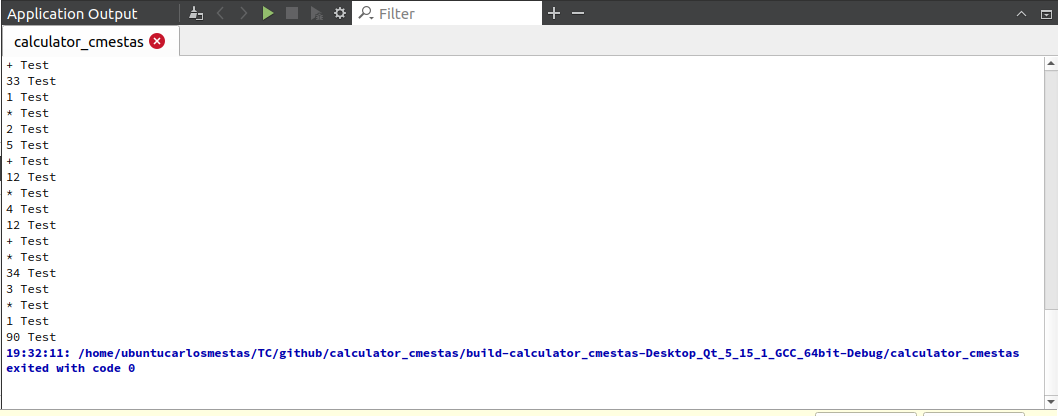
\includegraphics[width=1\textwidth]{screen2.png}
    \caption{Ejemplo del ingreso de datos en el árbol}
\end{figure}

\clearpage
\newpage

\end{document}
